\documentclass[12pt]{IEEEtran}
\usepackage[numbib]{tocbibind}
\usepackage{graphics}
\usepackage{caption}
\usepackage{subcaption}
\usepackage{graphicx}
\usepackage{float}
\usepackage{authblk}

\graphicspath{ {./images/} }
\bibliographystyle{IEEEtran}

\title{
    Wine Not? \\
    \large An exploration into the language of wine reviews
}
\author[1]{Austin Doolittle}
\author[1]{Maria Corina Cabezas}
\affil[1]{
    University of California, Berkeley
    \authorcr{\tt \{austin.doolittle, m.cabezas95\}@berkeley.edu}\vspace{1.5ex}
}

\begin{document}
\maketitle
\begin{abstract}
    Marketing heavily relies on language to persuade consumers into believing a product will improve their lives. The wine market is no different. With the number of online alcoholic beverage delivery services growing, it's now more important than ever for wine manufacturers to create enticing and interesting descriptions of their products. Our research involves the application of a variety of regression and classification models to professional wine reviews in an attempt to create useful models for evaluating the language of wine descriptions. We find that simple models work quite well with the problems we attempt to solve, yielding a positive outlook on the application of these elementary models on wine manufacturer's marketing initiatives.
\end{abstract}

\section{Introduction}
    Understanding user reviews is an essential part of any product branding and marketing strategy. Reviews can also provide companies with important feedback about the product and assist in decision making. Our goal is to use Natural Language Processing (NLP) algorithms to automate the process of analyzing wine reviews. We'll train a regression model that predicts the price of the wine and the score given to the wine by professional wine tasters, then test out new descriptions of wine to identify what their perceived score would be. We'll also create a classification task, first attempting to classify the wine by variety based on the language of the review, then creating a sentiment analysis model. This sentiment analysis model is particularly useful for wine companies trying to understand their own product reviews and see what blends are triggering more positive responses. 

    \begin{figure}
        \centering
        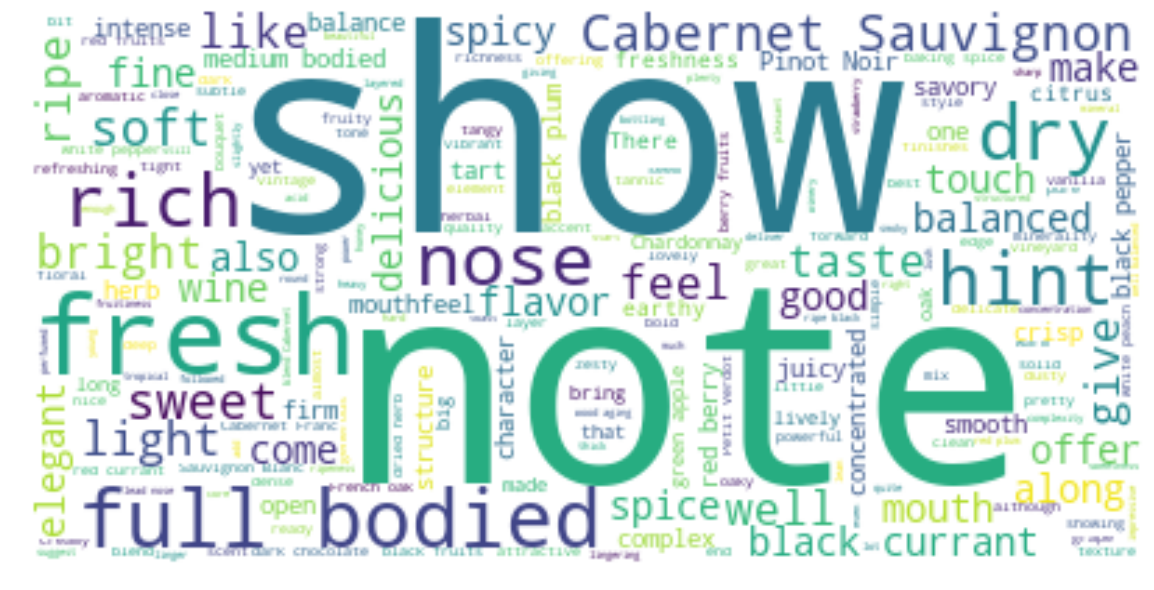
\includegraphics[width=\columnwidth]{wordcloud}
        \caption{Word cloud of the WineEnthusiast dataset's vocabulary. Generated with the wordcloud python package\cite{wordcloud}}
    \end{figure}

\section{Background}
    We intend to perform experiments with a wide array of different NLP algorithms to achieve our goal of understanding the luxury wine market via professional reviews. In order to determine which algorithms will be effective at these tasks, we should first identify the source and purpose of the dataset, then qualify the algorithms we intend to use with the problems that they solve.

\subsection{The Dataset}

\begin{figure}[b]
    \centering
    \begin{subfigure}{0.4\columnwidth}
    \small
    \begin{tabular}{ |l|r| }
        \hline
        Unigram & $r_{price}$ \\
        \hline
        \hline
        condrieu & 0.188 \\
	    enduring & 0.178 \\ 
	    reflects & 0.172 \\
	    component & 0.156 \\
	    perfectly & 0.154 \\
        \hline
        brusque & -0.093 \\
        enviable & -0.094 \\
        funky & -0.100 \\
        hyde & -0.105 \\
        weightless & -0.184 \\
        \hline
    \end{tabular}
    \end{subfigure}
    \begin{subfigure}{0.4\columnwidth}
    \small
    \begin{tabular}{ |l|r| }
        \hline
        Unigram & $r_{score}$ \\
        \hline
        \hline
        tufo & 0.149 \\
        heartland & 0.146 \\
        satisfying & 0.107 \\
        grower & 0.105 \\
        early & 0.103 \\
        \hline
        introductory & -0.063 \\
        drunk & -0.064 \\
        costs & -0.064 \\
        ager & -0.067 \\
        sangiovese & -0.068 \\
        \hline
    \end{tabular}
    \end{subfigure}
    \caption{Most extreme correlations between unigrams and their price and score}
    \label{correlations}
\end{figure}

\begin{figure*}
    \centering
    \begin{subfigure}[t]{0.4\textwidth}
        \centering
        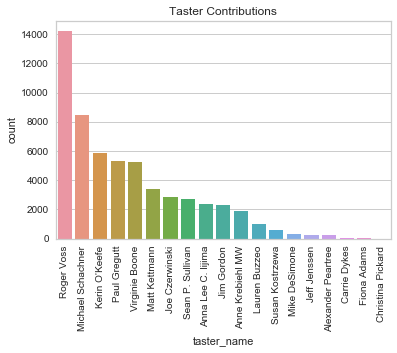
\includegraphics[width=\textwidth]{taster_contribution}
    \end{subfigure}
    \begin{subfigure}[t]{0.4\textwidth}
        \centering
        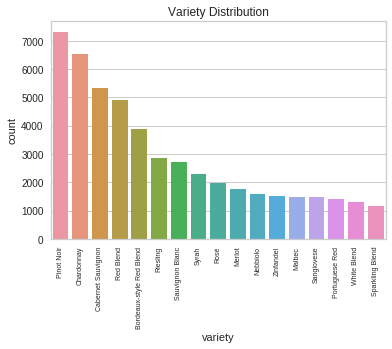
\includegraphics[width=\textwidth]{variety_distribution}
    \end{subfigure}
    \begin{subfigure}[t]{0.4\textwidth}
        \centering
        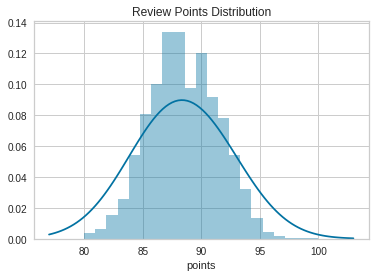
\includegraphics[width=\textwidth]{points_distribution}
    \end{subfigure}
    \begin{subfigure}[t]{0.4\textwidth}
        \centering
        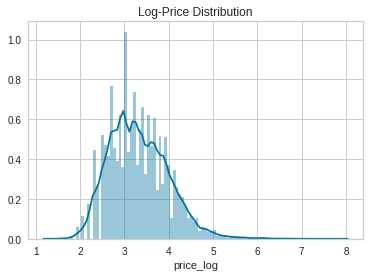
\includegraphics[width=\textwidth]{log_price_distribution}
    \end{subfigure}
    \caption{Distributions of different datapoints in the dataset}
    \label{data_distributions}
\end{figure*}


    The dataset consists of 130,000 wine reviews scraped from the WineEnthusiast Magazine's website in November of 2017. It includes the wine name, variety, winery name and location, price, and review text and score. The dataset was retrieved from Kaggle\cite{data}. \par
    Official wine scoring is done on a scale from 50 to 100, with a higher score indicating that the wine is superior\cite{wine_scoring}. WineEnthusiast will not publish reviews for any wine that scores less than 80 points, so the range of possible values for this specific dataset is 80 to 100. \par
    We should be mindful of the fact that there are 19 reviewers in our dataset, with one reviewer responsible for for $\frac{1}{10}$ of all reviews. This might indicate the dataset is not representative of the market itself, and we should be mindful of this bias when drawing conclusions from the data.
    We also observed that the distribution of varieties and countries of origins is not uniform, with most reviewed wines being Cabernet Sauvignon and coming from the United States. View Figure \ref{data_distributions} for more information regarding the distributions of different values in the dataset. \par
    Prior to the experiments outlined below, we split the data randomly into a train, test, and validation set. The sizes of these datasets are 71973, 23991, and 23991. \par
    Research in the NLP field has also shown that some difficult benchmark datasets contain latent bias that enable more complex models to perform very well without actually learning the task at hand. One example of research that identified this bias found that it was easily identifiable by observing the presence or absence of specific words in relation to their labels\cite{clever_hans}. In an attempt to identify this bias before our analysis, we conducted Pearson correlation studies on all unigrams, bigrams, and trigrams in our dataset. Figure \ref{correlations} displays the correlations between unigrams and the price and score labels\footnote{We include the results of correlation studies with bigrams and trigrams in Figure \ref{correlation_cont} in the appendix.}. We show here that we found no significant correlation on either end of the spectrum. This soothed fears of a biased dataset in this regard to these labels, and allowed the experiments to continue without major intervention.\footnote{More analysis was done in our preliminary investigation of this dataset than what is included in this section. Those results are included in the appendix for brevity.} \par

\subsection{Modeling}
    In many cases, linear models are able to solve regression problems with low error. While current advances in NLP have been proven to repeatedly outperform simpler, older models, we will include it in our analysis to ensure we don't blindly jump to using an overpowered, inefficient model. Linear models that we found to be useful are linear regression and logistic regression. We do use two other nonlinear, non-deep learning models in our research, which are random forest classifiers and multinomial naive bayes. \par
    These models require some feature vector as input. Three very simple methods of feature extraction from a corpus of text data are the age-old Bag-of-Words approach\cite{bag_of_words}, TF-IDF vectors, and Word2Vec embeddings \cite{word2vec}. We explore the application of both at different points in our research.\par
    Research has also shown that CNNs are capable of learning more complex relationships within blocks of text with the advantage of maintaining spatial relationships between tokens in the text\cite{cnn}. As with linear models, this model requires some input. Because CNNs are able to learn more complex relationships, it can be advantageous to use a more specialized method for creating our featureset. Creating an embedding matrix with learnable parameters allows for this featureset to be learned as if it was an additional parameter in the model.\par
    The absolute leader in the field of Natural Language Processing is the transformer layer. Of all implementations of this layer, the BERT model repeatedly yields state-of-the-art results in most NLP tasks\cite{bert}. We intend to use the embedding layer described above to generate learned vector embeddings for the input tokens in our use cases for BERT.

\section{Approach}
    As mentioned above, we set out to perform regression on the score and price of the wine, classification on the region and variety of wine, and sentiment analysis. The following outlines the approachs that we take for each of these problems.

\subsection{Regression}
    Before beginning training for regression, we preprocessed our text by removing all stop words, which in our implementation were a combination of NLTK's stopword collection, punctuation, and the top 10 most common words in the training dataset\footnote{A list of all stop words can found in Figure \ref{stop_words} in the Appendix.}. We used Mean Squared Error as both a loss function and an evaluation metric for all models. We normalize the score of the wine by scaling the values so the mean of the distribution is 0 and standard deviation is 1. We also take the base 10 log of the price and regress on that value. We'll now outline the three different types of models applied to this problem.\par
    The first was the SKLearn implementation of Linear Regression with a Bag-of-Words feature vector as input. The words were tokenized via the SKLearn $CountVectorizer$\cite{sklearn}, with all words being lowercased, split on spaces, and combined into ngrams of varying sizes, each of which are evaluated and shown in the results section. \par
    The next model is a CNN model. The model was implemented in Keras \cite{keras}, and consists of an embedding layer which creates an embedding of size 256, followed by 3 parallel convolutional layers with filter sizes of 3, 4, and 5. The output of those layers are concatenated and fed as input into a fully connected layer, with dropout of probability 0.1. The output of the model is a single scalar value that does not have an activation function. The text is preprocessed and tokenized with the Keras preprocessing library. \par
    Finally, our last model is a keras implementation of BERT. The implementation was found on GitHub and is authored by CyberZHG\cite{keras_bert}. Our BERT model has 12 transformers with 4 attention heads, a fully connected layer of size 100, and an embedding layer creating word vectors of size 256. The fully connected layers also have dropout applied with probability 0.05.

\subsection{Classification}
    Our classification analysis focused strictly on attempting to classify the variety of wine that was under review. To avoid underrepresentation among the more sparse classes, we only trained and evaluated the model on varieties with over 1,000 reviews in the train dataset, which ultimately was a list of 17 different varieties. The list of varieties include in this dataset can be found in Appendix \ref{variety_classes}. \par
    Our setup was very similar to our setup on the regression problem listed above. We remove stop words, and apply a linear model, a CNN, and BERT to the dataset. The only major difference is that instead of using a linear regression model, we use the SKLearn implementation of the logistic regression for our linear model benchmark\cite{sklearn}. We also use binary cross entropy for the loss function of the CNN and BERT model.

\subsection{Sentiment Analysis}
    Finally, we create a sentiment analysis model by turning the estimation of the score applied to the model from a regression problem into a classification problem. This is done by splitting the scores at 90, with values greater than or equal to 90 being labelled as the positive class, and vice-versa. The trained model is useful for wine companies trying to predict sentiment on new or existing products by looking at the specific aspects that are illiciting positive/negative emotions from people. \par
    Our experiments combined multiple different feature extraction methods and classification models. These are Bag-of-Words applied to a multinomial 
    Naive Bayes model, TF-IDF vectors applied to a Logistic Regression model, and finally Word2Vec applied to a random forest classifier. SKLearn was used for Bag-of-Words and TF-IDF feature extraction, as well as all models. We used the gensim implementation of Word2Vec\cite{gensim}. \par

\section{Results}
    We will now disclose the results of our experiments in Regression, Classification, and Sentiment Analysis.

\subsection{Regression}



    Figure \ref{regression_results} contains a table of the Mean Squared Error achieved by all models the regression task for both wine score and log-price. The BERT model performed best on the score regression task, however the CNN was very close behind. We also note that unigram Bag-of-Words with a Linear Regressor performed best of all the linear models. We expect this to be a result of the size of the dataset. There are many unique bigrams and trigrams in the dataset, which likely causes overtraining. \par
    For the wine price model, we similarly see that the BERT and CNN models performed best, but in this case the CNN edged ahead of the BERT model. We see a similar pattern here in regards to the ngram size, which supports our hypothesis. The results of running a sentence that test created for a fictional brand of wine can be seen in Figure \ref{regression_ex}.
\begin{figure}[H]
    \centering
    \resizebox{\columnwidth}{!}{%
    \begin{tabular}{ |l||r|r|  }
        \hline
        \multicolumn{3}{|c|}{Regression Results} \\
        \hline
        Model& Review Score (MSE) & Wine Price (MSE) \\
        \hline
        Unigram BoW   & 0.325          & 0.546 \\
        Bigram BoW    & 0.647          & 0.809 \\
        Trigram BoW   & 0.901          & 0.901 \\
        1-3gram BoW   & 0.460          & 0.805 \\
        \hline
        CNN                    & 0.285          & \textbf{0.499} \\
        \hline
        BERT                   & \textbf{0.283} & 0.513 \\
        \hline
    \end{tabular}}
    \caption{ Results of applying various regression models to the dataset. }
    \label{regression_results}
\end{figure}
\begin{figure*}
    \centering
    \begin{subfigure}{\columnwidth}
        \centering
        \textbf{Tantalizing the taste buds, Five Oaks brand chardonnay is truly 
        a taste sensation. Few wines are this full bodied while also leaving some
        room for the imagination.}
        \caption{A test sentence ran over all other models}
    \end{subfigure}
    \begin{subfigure}{\columnwidth}
        \centering
        \resizebox{\columnwidth}{!}{%
        \begin{tabular}{ |l||r|r|  }
            \hline
            Model& Review Score (Points) & Wine Price (Dollars) \\
            \hline
            Unigram BoW   & 87.3         & 25.5 \\
            Bigram BoW    & 86.9          & 18.1 \\
            Trigram BoW   & 80.9         & 13.9 \\
            1-3gram BoW   & 85.5          & 7.5 \\
            \hline
            CNN                    & 87.5        & 12.2 \\
            \hline
            BERT                   & 86.1 &  8.9 \\
            \hline
        \end{tabular}}
        \caption{The predictions of the model on the test sentence}
    \end{subfigure}
    \caption{ The result of applying the above text to the various models}
    \label{regression_ex}
\end{figure*}

\subsection{Classification}

    Figure \ref{classification_results} shows the accuracy achieved by each model applied to the variety classification task. Logistic regression in this case performed quite well when compared to the more complex models that were tested. It seems that this data is close to being linearly seperable. This goes against our observation of the correlation of certain words against price and score. In future analysis, we intend to also investigate correlation of tokens with categorical variables, as there may be latent bias present in those values as well. Ultimately the top performing model was BERT, as expected. \par
\begin{figure}[H]
    \centering
    \begin{tabular}{ |l|r|  }
        \hline
        \multicolumn{2}{|c|}{Variety Classification} \\
        \hline
        Model & Accuracy \\
        \hline
        Unigram BoW   & 0.67 \\
        Bigram BoW   & 0.60 \\
        Trigram BoW  & 0.46 \\
        1-3gram BoW   & 0.74 \\
        \hline
        CNN                    & 0.52 \\
        \hline
        BERT                   & \textbf{0.79} \\
        \hline
    \end{tabular}
    \caption{ Results of various regression models applied to the dataset. }
    \label{classification_results}
\end{figure}
    It is quite interesting that the CNN had the worst performance of all models in this experiment. We were not able to come up with a reasonable explanation for this, more testing is likely required to come to a strong hypothesis on why this is.\par



\subsection{Sentiment Analysis}
    Model performance on the development dataset can be viewed in Figure \ref{sentiment_results}. Similar to our variety classification task, this classification is best accomplished by a linear classifier. An examination of the coefficients indicates why this may be. In Figure \ref{sentiment_coefficients}, we see that the largest coefficients were assigned to numbers. Our preprocessing for these models did not include the condensing of numbers into a single token. We expect that this caused our model to overtrain on these values and, due to the relatively small problem domain and size of the dataset, caused the model to be rather successful on the dev dataset. In future experiments, we intend to add the condensing of numeric digits to a single token to mitigate the effect of low frequency tokens.

\begin{figure}[H]
\centering
    \resizebox{\columnwidth}{!}{%
    \begin{tabular}{ |l|l|r|  }
        \hline
        \multicolumn{3}{|c|}{Sentiment Classification Results} \\
        \hline
        Feature Extraction & Model & Accuracy \\
        \hline
        Bag-of-Words & Multinomial Naive Bayes & 0.82 \\
        TF-IDF Vectors & Logistic Regression & \textbf{0.85} \\
        Word2Vec   & Random Forest & 0.74 \\
        \hline
    \end{tabular}}
    \caption{ The performance of our sentiment classification models }
    \label{sentiment_results}
\end{figure}

\begin{figure}[H]
    \centering
    \begin{tabular}{ |l|r| }
        \hline
        \multicolumn{2}{|c|}{Sentiment Coefficients} \\
        \hline
        Token & Coefficient \\
        \hline
        2025 & 8.32 \\
        92 & 7.70 \\
        2030 & 7.40 \\
        2022 & 7.15 \\
        beautiful & 6.73 \\
        \hline
        89 & -3.83 \\
        straightforward & -4.42 \\
        lacks & -4.70 \\
        easy & -4.71 \\
        simple & -6.07 \\
        \hline
    \end{tabular}
    \caption{Most extreme coefficients from the logistic regression sentiment analysis model}
    \label{sentiment_coefficients}
\end{figure}
\section{Conclusion}
    Our approach allows for wine manufacturers to make intelligent decisions about the language used in their marketing material promoting their product, and allows them to know how their language makes their product distinct. While our research was comprehensive, we feel there is still much ground to cover. Further analysis includes applying clustering algorithms to identify groupings of similar wines based on their reviews. This information would be useful for targetted marketing campaigns with the ultimate goal of grabbing the attention of new customers. Our approach is also purely reactionary. The application of generative models would allow manufacturers to automate the description process of their wine, further optimizing their marketing approaches. Ultimately, there are plenty more insights to extract from this dataset and from the wine market itself.

\bibliography{final_report}

\newpage
\section{Appendix}

\begin{figure}[h]
    Bordeaux-style Red Blend, Cabernet Sauvignon, Chardonnay, Malbec, Merlot, Nebbiolo, Pinot Noir, Portuguese Red, Red Blend, Riesling, Rosé, Sangiovese, Sauvignon Blanc, Sparkling Blend, Syrah, White Blend, and Zinfandel
    \caption{Variety Classes}
    \label{variety_classes}
\end{figure}

\begin{figure}[h]
    \centering
    \begin{subfigure}[t]{\columnwidth}
        \centering
        \begin{tabular}{ lr  }
            \hline
            Unigram & Count \\
            \hline
            black  & 15967 \\
            ripe   & 14979 \\
            red    & 11949 \\
            spice  & 10658 \\
            notes  & 10438
        \end{tabular}
        \caption{ Top five unigram counts}
    \end{subfigure}
    \begin{subfigure}[t]{\columnwidth}
        \centering
        \begin{tabular}{ lr  }
            \hline
            Bigram & Count \\
            \hline
            full bodied & 3786 \\
            cabernet sauvignon & 2931 \\
            medium bodied & 1794 \\
            pinot noir & 1757 \\
            red berry & 1710
        \end{tabular}
        \caption{ Top five bigram counts}
    \end{subfigure}
    \begin{subfigure}[t]{\columnwidth}
        \centering
        \begin{tabular}{ lr  }
            \hline
            Trigram & Count \\
            \hline
            new french oak  & 436 \\
            red berry fruits & 381 \\
            blend cabernet sauvignon & 322 \\
            cabernet sauvignon merlot & 309 \\
            merlot cabernet sauvignon & 228 
        \end{tabular}
        \caption{ Top five trigram counts} 
    \end{subfigure} 
    \caption{NGram Distributions}
    \label{ngram_distribution}
\end{figure}

\begin{figure}[h]
    \centering
    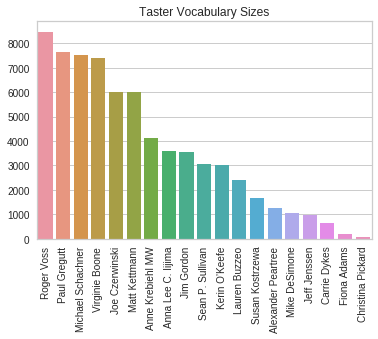
\includegraphics[width=\columnwidth]{taster_vocabularies}
    \caption{Taster Vocabulary Distributions}
\end{figure}

\begin{figure*}
    \centering
    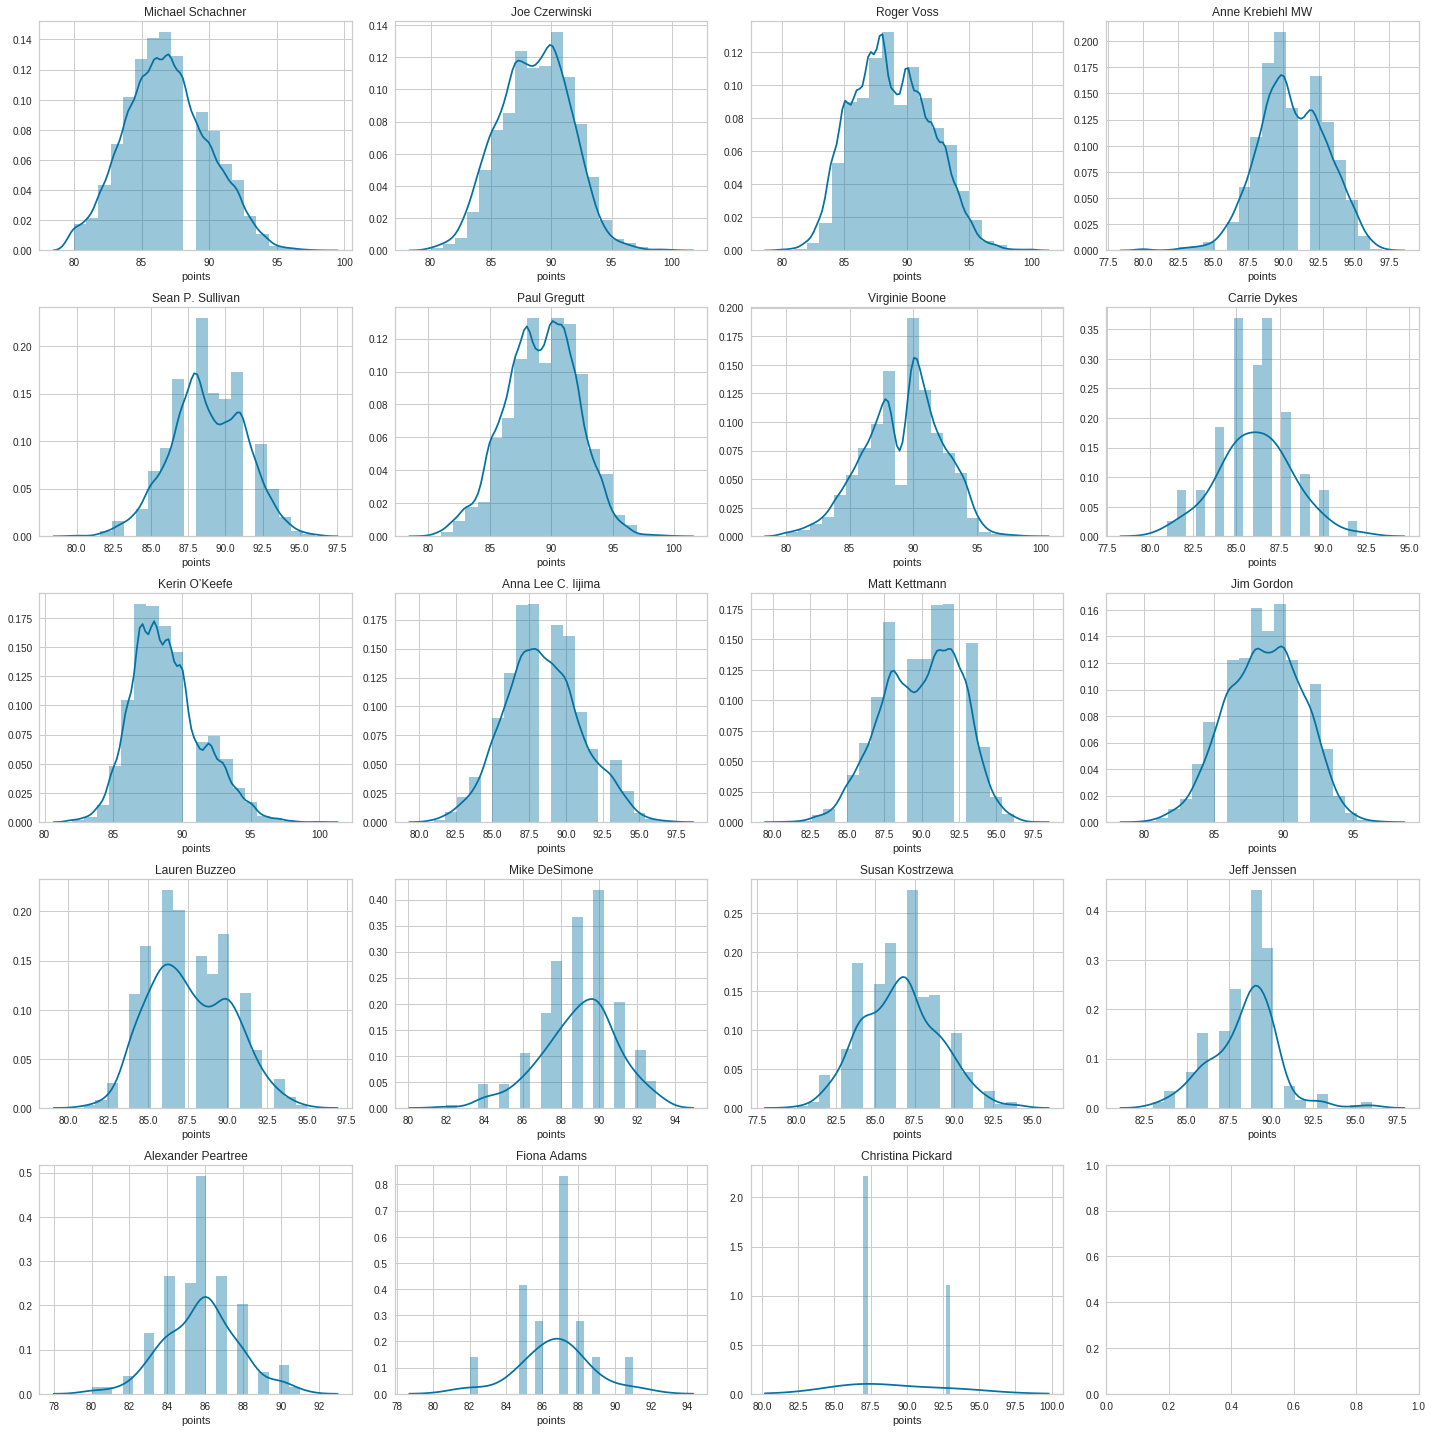
\includegraphics[width=\linewidth]{taster_score_distributions}
    \caption{Taster Score Distributions}
\end{figure*}

\begin{figure*}[h]
    \centering
    \begin{subfigure}{\columnwidth}
    \centering
    \small
    \begin{tabular}{ |l|r| }
        \hline
        Bigram & $r_{price}$ \\
        \hline
        \hline
        character suggests & 0.0923 \\
	    tea notes & 0.078 \\
	    blend offers & 0.077 \\
	    strongly herbal & 0.075 \\
	    berry end & 0.067 \\
        \hline
        good well & -0.049 \\
        cola coffee & -0.049 \\
        offers impressive & -0.052 \\
        easy pinot & -0.052 \\
        cedar mocha & -0.053 \\
        \hline
    \end{tabular}
    \end{subfigure}
    \begin{subfigure}{\columnwidth}
    \centering
    \small
    \begin{tabular}{ |l|r| }
        \hline
        Bigram & $r_{score}$ \\
        \hline
        \hline
        would perfect & 0.140 \\
	    extremely ripe & 0.119 \\ 
	    fruits light & 0.083 \\
	    delivers thick & 0.082 \\
	    cranberry juice & 0.082 \\
        \hline
        alcohol well &  -0.028 \\
        earth black &  -0.035 \\
        bodied still & -0.036 \\
        note signals & -0.039 \\
        pear along & -0.042 \\
        \hline
    \end{tabular}
    \end{subfigure}
    \begin{subfigure}{\columnwidth}
    \centering
    \small
    \begin{tabular}{ |l|r| }
        \hline
        Trigram & $r_{price}$ \\
        \hline
        \hline

        100 cabernet sauvignon & 0.056 \\
        creamy white peach & 0.046 \\
        fresh fruity light & 0.046 \\
        cabernet sauvignon 30 & 0.043 \\
        cabernet franc syrah & 0.043 \\
        \hline
        red plum skin & -0.023 \\
        apple meyer lemon & -0.022 \\
        apple tangerine zest & -0.022 \\
        touch orange zest & -0.021 \\
        cassis red currant & -0.021 \\

        \hline
    \end{tabular}
    \end{subfigure}
    \begin{subfigure}{\columnwidth}
    \centering
    \small
    \begin{tabular}{ |l|r| }
        \hline
        Trigram & $r_{score}$ \\
        \hline
        \hline
        fresh lemon lime & 0.093 \\
        high toned notes & 0.052 \\
        opens leafy underbrush & 0.050 \\
        third new french & 0.046 \\
        least five years & 0.046 \\
        \hline
        fresh green herbs & -0.014 \\
        notes buttered toast & -0.013 \\
        fuller bodied style & -0.012 \\
        need time come & -0.012 \\
        herb take center & -0.011 \\
        \hline
    \end{tabular}
    \end{subfigure}
    \caption{Correlation analysis of bigrams and trigrams}
    \label{correlation_cont}
\end{figure*}


\begin{figure*}
    \centering
    \resizebox{\linewidth}{!}{%
    \begin{tabular}{|c|c|c|c|c|c|c|c|c|c|}
        \hline
        \multicolumn{10}{|c|}{Stop Words} \\
        \hline
        your & weren & don & having & before &finish & didn & ( & in & does \\
        \hline
        d & you'll & needn & yourself & what & under & than & ; & \textasciitilde & any \\
        \hline
        nor & from & why & needn't & weren't &    both & up & further & during & there \\
        \hline
        them & at & wasn't & same & s &    $<$ & just & below & it & again \\
        \hline
        didn't & aromas & those & haven & ma &    now & mustn't & if & itself & him \\
        \hline
        has & no & | & which & our &    was & i & such & drink & for \\
        \hline
        can & o & over & how & with &    this & my & be & ll & \textbackslash \\
        \hline
        ` & yourselves & aren't & once & hadn't &    after & you & do & here & \& \\
        \hline
        me & where & about & don't & by &    flavors & then & themselves & own & hadn \\
        \hline
        hers & doesn & her & . & is &    ? & down & tannins & wouldn & {[} \\
        \hline
        of & aren & been & or & y &    few & shouldn & through & : & between \\
        \hline
        who & have & mightn't & / & isn &    it's & when & he & and & against \\
        \hline
        an & herself & ve & = & + &    ] & \{ & very & a & couldn't \\
        \hline
        wasn & t & wouldn't & \# & ) &    their & out & \_ & but & because \\
        \hline
        ain & won & yours & couldn & shouldn't &    \textasciicircum & these & isn't & they & into \\
        \hline
        myself & were & m & shan & only &    all & his & that'll & had & she's \\
        \hline
        as & haven't & > & its & so &    cherry & more & too & each & did \\
        \hline
        \$ & she & ourselves & am & should've &    whom & you're & doing & shan't & * \\
        \hline
        are & the & until & himself & being &    you'd & other & will & mustn & \% \\
        \hline
        re & that & - & we & you've &    not & acidity & won't & mightn & " \\
        \hline
        ours & doesn't & \} & above & ! &    some & while & ' & fruit & wine \\
        \hline
        @ & hasn & most & to & on &    , & off & should & hasn't & palate \\
        \hline
        theirs & & & & & & & & & \\
        \hline
    \end{tabular}}
    \caption{Stop words that were removed during text preprocessing}
    \label{stop_words}
    \end{figure*}
\end{document}
